\documentclass[a4paper,12pt]{article}

\usepackage{amsmath,amssymb,amsfonts}
\usepackage{makecell}
\usepackage{multirow}
\usepackage[utf8]{inputenc}
\usepackage[brazil]{babel}
\usepackage{graphicx}
\usepackage[bookmarks]{hyperref}
\usepackage{bookmark}
\usepackage{listings}
\usepackage{float}
\usepackage{pgffor}
\usepackage{lmodern}
\usepackage{textcomp}
\usepackage{amsmath}
\usepackage[separate-uncertainty=true]{siunitx}
\usepackage{xcolor}
\usepackage[most]{tcolorbox}



\newcommand{\nonumsection}[1]{%
  \section*{#1}%
  \addcontentsline{toc}{section}{#1}%
}
\newcommand{\nonumsubsection}[1]{%
  \subsection*{#1}%
  \addcontentsline{toc}{subsection}{#1}%
}


\title{Trabalho 2 \\ Disciplina de Reconhecimento de Padrões}
\author{Davi de Lima Cruz \\ mat: 474377}
\date{\today}

\begin{document}

\clearpage\maketitle
\thispagestyle{empty}
\nonumsection{Introdução}
O objetivo deste trabalho é comparar diferentes classificadores de reconhecimento de padrões aplicados a imagens de rostos de pessoas.
Serão utilizados classificadores como Quadrático, MaxCorr, DMC e 1-KK, além de aplicar normalizações e PCA (Análise de Componentes Principais).
O código utilizado para este trabalho está disponível no repositório do GitHub: \url{https://github.com/Davi0Cruz/Reconhecimento_de_Padroes}.
Um resumo teórico sobre cada classificador utilizado será apresentado:
\begin{itemize}
    \item \textbf{Classificador Quadrático}: Presupoem que os predirores seguem uma distribuição gaussiana multivariada,
    a partir disso calcula a matrix de covariância e a média de cada classe, e para testar ele ver qual das classes tem a
    distribuição que deu o maior valor de densidade de probabilidade ou menor discriminante.
    \item \textbf{A variante 1 do classificador Quadrático} é uma versão que adiciona uma pequena constante $\lambda$ à diagonal da matriz de covariância, sendo equivalente a adicionar um pouco de ruído aos dados.
    \item \textbf{A variante 2 do classificador Quadrático} pondera as matrizes de covariância de todas as classes e calcula a densidade de probabilidade
    a partir disso.
    \item \textbf{A variante 3 do classificador Quadrático} é um meio termo entre o Classificador Quadrático e a variante 2, ele interpola as matrizes de covariância
    de cada classe com a gerada pela variante 2.
    \item \textbf{A variante 4 do classificador Quadrático} considera apenas a diagonal da matriz de covariância, ou seja, assume que as variáveis são independentes.
     A vantagem disso é que compotacionalmente é muito mais barato inverter uma matriz diagonal do que uma matriz completa.
    \item \textbf{Classificador MaxCorr}: É um classificador baseado na correlação, é calculada a média de cada classe é comparada qual média tem a maior correlação com o vetor de teste.
    \item \textbf{Classificador DMC}: É um classificador baseado na distância dos centroides, onde a distância é medida em relação à média de cada classe.
    \item \textbf{Classificador 1-KK}: É um classificador baseado no KNN (K-Nearest Neighbors), onde K=1, ou seja, ele pega o vizinho mais próximo e atribui a classe desse vizinho ao preditor.
\end{itemize}

\nonumsection{Atividade 1}
\begin{tcolorbox}[colback=blue!5!white, colframe=blue!75!black]
    Abrir e executar o arquivo face\_preprocessing\_column.m sem aplicação do
PCA. Ou seja, comentar as linhas 56-60. Escolha as dimensões para redução das imagens
na linha 37. Note que quanto maior os valores da redução, maior será a dimensão dos
vetores de atributos após a vetorização das imagens e, obviamente, maior será o tempo de
treinamento/teste dos classificadores.
\end{tcolorbox}

O script foi executado com o tamanho da imagem sendo 20x20~pixels,
pois mais do que isso aumentava bastante o tempo de execução. 
\nonumsection{Atividade 2}
\begin{tcolorbox}[colback=blue!5!white, colframe=blue!75!black]
    Abrir e executar o arquivo compara\_todos.m usando Ptrain = 80; ou seja,
80\% dos vetores de atributos serão usados para treinar os classificadores. Faça também
Nr = 50 (número de repetições independentes de treino/teste).
 Executar o código e preencher a tabela de estatísticas de desempenho abaixo. A figura de mérito é a taxa de
acerto do classificador, determinando-se suas estatísticas descritivas ao final das 50 rodadas
independentes, tais como valor médio, desvio padrão, valores mínimos/máximos e mediana.
\end{tcolorbox}
Foram implementadas as normalizações ZScore, [0, 1] e [-1, 1] para cada Classificador MaxCorr, DMC e 1-KK.
Para o 1-KK e o DMC, o melhor foi sem normalização,
para o MaxCorr foi a [0, 1].

Além disso, para comparar melhor os resultados colocamos uma seed referente a cada rodada de execução em todos os algoritmos,
ou seja a divisão entre treino e teste foi a mesma para todos os algoritmos,
essa separação se repete para as próximas comparações.

Outra modificação feita foi mudar a forma como era calculado o discriminante dos classificadores Quadrático e suas variantes,
O termo $\ln(\det(C))$ acabava tendo o determinante zerado, o que fazia com que o discriminante ficasse indefinido,
então foram calculados os autovetores e autovalores da matriz de covariância, e substituímos essa parte pela soma dos logaritmos dos autovalores.
Como os autovetores já foram calculados, aproveitamos eles para calcular a matrix inversa da matriz de covariância.

\begin{table}[H]
\centering
\resizebox{0.8\textwidth}{!}{
\begin{tabular}{|c|c|c|c|c|c|c|}%
\hline%
\multirow{2}{*}{\textbf{Classificador}}&\multirow{2}{*}{\textbf{Média}}&\multirow{2}{*}{\textbf{Mínimo}}&\multirow{2}{*}{\textbf{Máximo}}&\multirow{2}{*}{\textbf{Mediana}}&\textbf{Desvio}&\textbf{Tempo de}\\%
&&&&&\textbf{Padrão}&\textbf{Execução (s)}\\%
\hline%
\hline%
\textbf{Quadrático}&16.727&3.030&36.364&15.152&7.198&56.855\\%
\hline%
\textbf{Variante 1}&80.121&69.697&96.970&78.788&6.188&55.924\\%
\hline%
\textbf{Variante 2}&44.000&27.273&66.667&42.424&10.194&7.606\\%
\hline%
\textbf{Variante 3}&36.970&15.152&51.515&36.364&9.081&58.247\\%
\hline%
\textbf{Variante 4}&15.939&0.000&30.303&15.152&7.518&11.798\\%
\hline%
\textbf{MaxCorr}&80.364&66.667&93.939&80.303&6.037&0.481\\%
\hline%
\textbf{DMC}&78.909&66.667&93.939&78.788&6.242&0.256\\%
\hline%
\textbf{1{-}KK}&78.848&60.606&96.970&78.788&7.485&2.013\\%
\hline%
\hline%
\end{tabular}
}
\caption{Tabela de resultados sem a aplicação de PCA}
\end{table}

\begin{figure}[H]
\centering
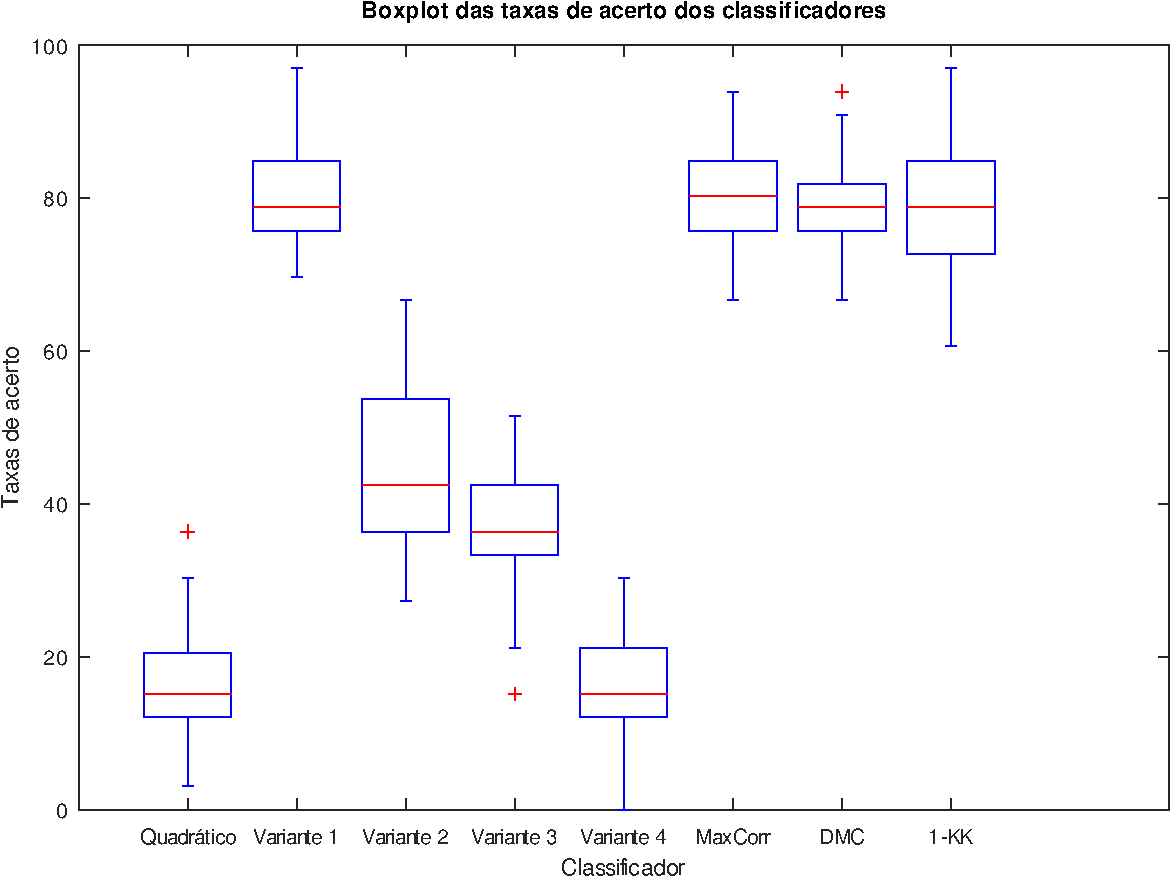
\includegraphics[width=0.6\textwidth]{figs/boxplot_sem_pca.pdf}
\caption{Boxplot dos resultados sem a aplicação de PCA}
\end{figure}

\nonumsubsection{Questão 1}
\begin{tcolorbox}[colback=blue!5!white, colframe=blue!75!black]
    O que se pode concluir sobre os desempenhos dos classificadores avaliados?
\end{tcolorbox}
Para os classificadores Quadrático e suas variantes,
as matrizes de covariância apresentaram o warning sobre o condicionamento, menos para a variante 1.
O que fez com que os resultados fossem muito ruins para esses classificadores.
Já os outro métodos tiveram resultados melhores e mais rápidos, tendo o de MaxCorr como o melhor resultado médio com 80\% de acerto.

\nonumsubsection{Questão 2}
\begin{tcolorbox}[colback=blue!5!white, colframe=blue!75!black]
    Qual deles teve o melhor desempenho em relação à taxa de acerto? E em
relação ao tempo?
\end{tcolorbox}
O classificador que teve o melhor resultado médio foi o de MaxCorr com 80\% de acerto.
Quanto ao tempo de execução, o DMC foi o mais rápido, levando apenas 0.25 segundos.

\nonumsubsection{Questão 3}
\begin{tcolorbox}[colback=blue!5!white, colframe=blue!75!black]
    Houve problemas de inversão das matrizes de covariância? Se sim, para quais
classificadores? Este problema foi contornado por alguma das variantes avaliadas? Se
sim, descreva sucintamente o mecanismo usado para resolvê-lo.
\end{tcolorbox}
Os classificadores Quadrático e suas variantes não conseguiram inverter suas matrizes por conta do condicionamento,
o que fez com que os resultados fossem muito ruins. A variante 1 conseguiu contornar isso com a regularização,
lembrando que essa variante 1 funciona por meio da adição de uma diagonal com um valor pequeno (0.01) à matriz de covariância,
isso ajuda a dar independência linear entre as linhas da matriz.

\nonumsection{Atividade 3}
\begin{tcolorbox}[colback=blue!5!white, colframe=blue!75!black]
    Executar o arquivo face preprocessing column.m com aplicação do PCA.
Ou seja, descomentar as linhas 56-60. Faça q = 400 ou q = 900 na linha 57, a depender
do redimensionamento das imagens escolhido na Atividade 1. Note que para este valor
de q, a aplicação de PCA não conduz a uma redução da dimensionalidade dos vetores de
atributos, mas sim promove apenas a diagonalização da matriz de covariância dos dados
transformados. Em outras palavras, os atributos para o novo conjunto de dados Z são
descorrelacionados entre si.
\end{tcolorbox}
\nonumsection{Atividade 4}
\begin{tcolorbox}[colback=blue!5!white, colframe=blue!75!black]
    Executar novamente a Atividade 2, preenchendo a tabela de desempenho
abaixo.
\end{tcolorbox}
\begin{figure}[H]
\centering
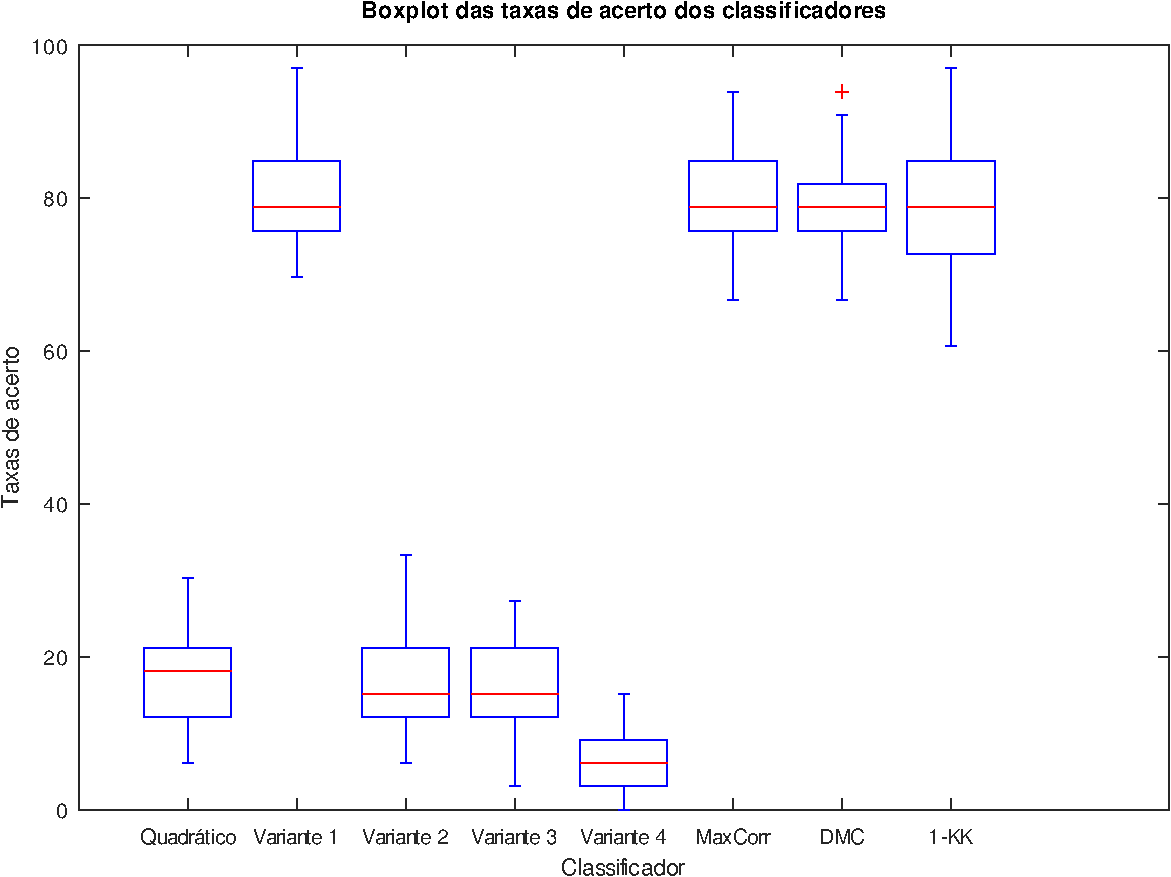
\includegraphics[width=0.7\textwidth]{figs/boxplot_pca_sem_red.pdf}
\caption{Boxplot dos resultados com PCA (sem redução)}
\end{figure}

\begin{table}[H]
\centering
\resizebox{0.9\textwidth}{!}{
\begin{tabular}{|c|c|c|c|c|c|c|}%
\hline%
\multirow{2}{*}{\textbf{Classificador}}&\multirow{2}{*}{\textbf{Média}}&\multirow{2}{*}{\textbf{Mínimo}}&\multirow{2}{*}{\textbf{Máximo}}&\multirow{2}{*}{\textbf{Mediana}}&\textbf{Desvio}&\textbf{Tempo de}\\%
&&&&&\textbf{Padrão}&\textbf{Execução (s)}\\%
\hline%
\hline%
\textbf{Quadrático}&16.848&6.061&30.303&18.182&5.972&52.371\\%
\hline%
\textbf{Variante 1}&80.121&69.697&96.970&78.788&6.188&49.189\\%
\hline%
\textbf{Variante 2}&16.364&6.061&33.333&15.152&7.113&4.869\\%
\hline%
\textbf{Variante 3}&15.818&3.030&27.273&15.152&5.817&48.728\\%
\hline%
\textbf{Variante 4}&6.061&0.000&15.152&6.061&3.463&11.664\\%
\hline%
\textbf{MaxCorr}&80.182&66.667&93.939&78.788&6.159&0.320\\%
\hline%
\textbf{DMC}&78.909&66.667&93.939&78.788&6.242&0.209\\%
\hline%
\textbf{1{-}KK}&78.848&60.606&96.970&78.788&7.485&1.867\\%
\hline%
\hline%
\end{tabular}
}
\caption{Resultados com PCA (sem redução)}
\end{table}

\nonumsubsection{Questão 4}
\begin{tcolorbox}[colback=blue!5!white, colframe=blue!75!black]
   $(i)$ O que se pode concluir sobre os desempenhos dos classificadores avaliados?
Houve alguma mudança (melhora ou piora) nos desempenhos dos classificadores
avaliados em relação à tabela anterior? $(ii)$ Note que, com a aplicação de PCA aos
dados originais, a matriz de covariância dos dados transformados é diagonal. Isso
faz com que o classificador quadrático e a Variante 4 sejam teoricamente equivalentes.
Estes classificadores tiveram de fato desempenho equivalente nos experimentos
relacionados?
\end{tcolorbox}
\begin{itemize}
    \item Os classificadores quadráticos que não tiveram regularização todos pioraram muito seus resultados,
    basicamente as matrizes estavam todoas mal condicionadas, o que fez com que os resultados fossem muito ruins.
    \item Não, pois note que a PCA foi applicada em todo o conjunto de dados, tanto de teste quanto de treino.
     Quando os dados de treino são selecionados, a matriz de covariância não é mesma que foi diagonalizada pela PCA.
    Essa pequena mudança foi suficiente para que o condicionamento das matrizes de covariância fosse piorado.
\end{itemize}
A variante 1 do classificador Quadrático se beneficiou bastante do PCA, pois conseguiu inverter a matriz de covariância.
\nonumsection{Atividade 5}
\begin{tcolorbox}[colback=blue!5!white, colframe=blue!75!black]
    Com base na figura gerada durante a execução da atividade anterior, que
mostra a variância explicada acumulada em função do número de componentes conside-
rado, escolher um valor para q que preserve pelo menos 98\% da informação (i.e., variância)
dos dados originais. O valor de q adequado pode ser escolhido visualizando o conteúdo do
vetor V Eq, como sendo aquela componente cujo valor é maior que 98\%. Executar o ar-
quivo face preprocessing column.m com aplicação do PCA para o valor de q escolhido.
Note que para este valor de q, a aplicação de PCA conduz a uma redução da dimensiona-
lidade dos vetores de atributos, além de promover a descorrelação dos atributos dos dados
transformados.
\end{tcolorbox}

\nonumsubsection{Questão 5}
\begin{tcolorbox}[colback=blue!5!white, colframe=blue!75!black]
    Qual foi a dimensão de redução q escolhida, de modo a preservar 98\% da
informação do conjunto de dados original?
\end{tcolorbox}
\begin{figure}[H]
    \centering
    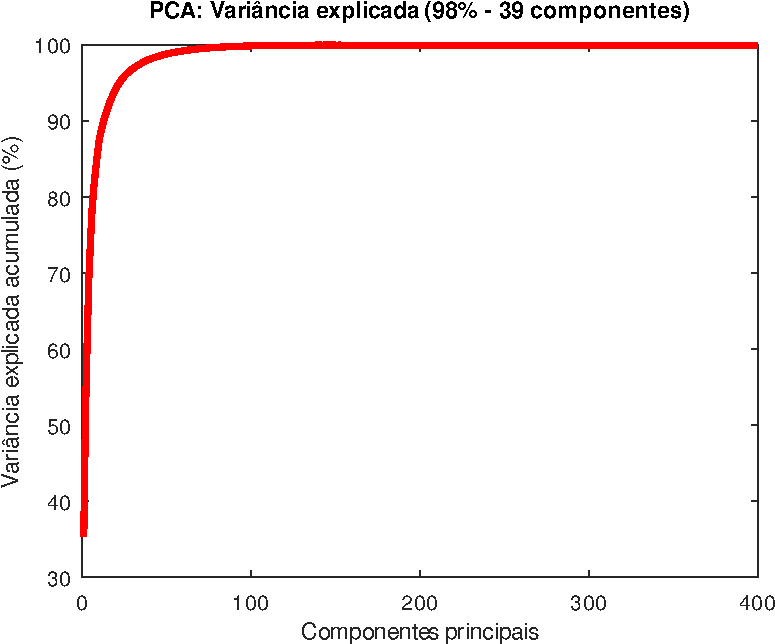
\includegraphics[width=0.5\textwidth]{figs/pca_variance.pdf}
    \caption{Variância acumulada em função do número de componentes.}
\end{figure}
Podemos ver que a partir de 39 componentes já temos mais de 98\% da variância acumulada,
então escolhemos $q = 39$.

\nonumsection{Atividade 6}
\begin{tcolorbox}[colback=blue!5!white, colframe=blue!75!black]
    Com base no valor escolhido para q na Atividade 5 e no conjunto de dados
gerados correspondente, preencha a tabela de desempenho abaixo.
\end{tcolorbox}

\begin{table}[H]
    \centering
    \resizebox{0.9\textwidth}{!}{
    \begin{tabular}{|c|c|c|c|c|c|c|}%
\hline%
\multirow{2}{*}{\textbf{Classificador}}&\multirow{2}{*}{\textbf{Média}}&\multirow{2}{*}{\textbf{Mínimo}}&\multirow{2}{*}{\textbf{Máximo}}&\multirow{2}{*}{\textbf{Mediana}}&\textbf{Desvio}&\textbf{Tempo de}\\%
&&&&&\textbf{Padrão}&\textbf{Execução (s)}\\%
\hline%
\hline%
\textbf{Quadrático}&54.667&33.333&78.788&54.545&9.562&0.568\\%
\hline%
\textbf{Variante 1}&79.273&66.667&96.970&78.788&6.576&0.579\\%
\hline%
\textbf{Variante 2}&95.576&84.848&100.000&96.970&3.735&0.416\\%
\hline%
\textbf{Variante 3}&95.091&87.879&100.000&95.455&3.511&0.596\\%
\hline%
\textbf{Variante 4}&76.121&63.636&93.939&75.758&7.363&0.495\\%
\hline%
\textbf{MaxCorr}&95.152&84.848&100.000&96.970&4.329&0.217\\%
\hline%
\textbf{DMC}&92.667&81.818&100.000&93.939&4.977&0.168\\%
\hline%
\textbf{1{-}KK}&87.212&72.727&96.970&87.879&5.687&1.451\\%
\hline%
\hline%
\end{tabular}
    }
    \caption{Resultados com PCA (com redução)}
\end{table}

\begin{figure}[H]
    \centering
    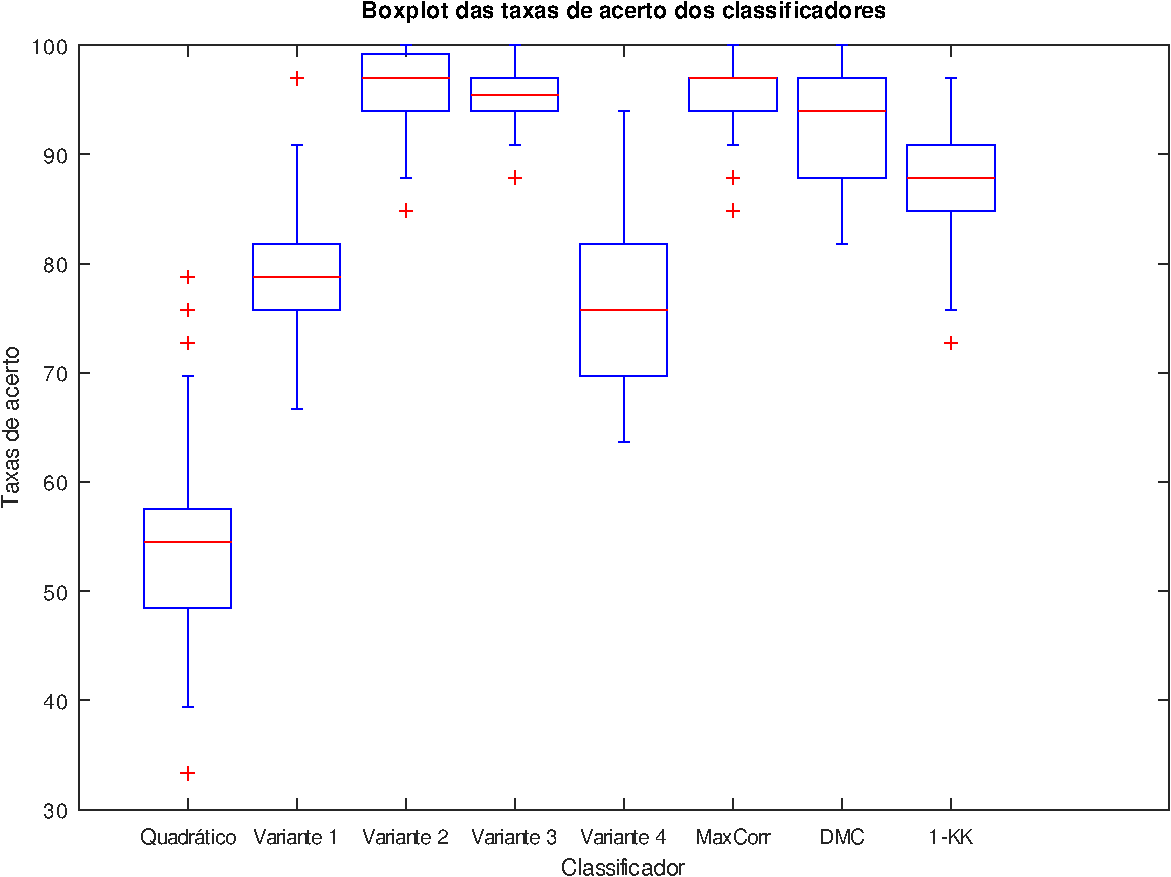
\includegraphics[width=0.7\textwidth]{figs/boxplot_pca_red.pdf}
    \caption{Boxplot dos resultados com PCA (com redução)}
\end{figure}
\nonumsubsection{Questão 6}
\begin{tcolorbox}[colback=blue!5!white, colframe=blue!75!black]
    O que se pode concluir sobre os desempenhos dos classificadores avaliados
com a realização da redução de dimensionalidade via PCA? Houve alguma mudança
(melhora ou piora) nos desempenhos dos classificadores avaliados em relação à tabela
anterior? Quais classificadores pioraram/melhoraram de desempenho com a redução
de dimensionalidade via PCA?
\end{tcolorbox}
Com a redução de dimensionalidade, os classificadores Quadrático e suas variantes tiveram uma melhora significativa,
pois as matrizes de covariância ficaram muito mais bem condicionadas, o que fez com que os resultados fossem muito melhores.
O classificador quadrático ainda teve dificuldade de condicionamento e por isso não teve resultados tão bons quanto os outros classificadores.

Os classificadores MaxCorr, DMC e 1-KK tiveram uma melhora significativa nos resultados.
Além disso, o tempo de execução dos classificadores Quadrático e suas variantes diminuiu abruptamente, pois o número de atributos foi reduzido.
Chegando a concorrer com os outro classificadores baseados em distância euclidiana.


\nonumsection{Atividade 7}
\begin{tcolorbox}[colback=blue!5!white, colframe=blue!75!black]
    Repita a Atividade 6, porém aplicando a transformação de BOX-COX
ao conjunto de dados original antes de aplicar PCA.
\end{tcolorbox}

\begin{table}[H]
    \centering
    \resizebox{0.9\textwidth}{!}{
    \begin{tabular}{|c|c|c|c|c|c|c|}%
\hline%
\multirow{2}{*}{\textbf{Classificador}}&\multirow{2}{*}{\textbf{Média}}&\multirow{2}{*}{\textbf{Mínimo}}&\multirow{2}{*}{\textbf{Máximo}}&\multirow{2}{*}{\textbf{Mediana}}&\textbf{Desvio}&\textbf{Tempo de}\\%
&&&&&\textbf{Padrão}&\textbf{Execução (s)}\\%
\hline%
\hline%
\textbf{Quadrático}&49.758&36.364&72.727&48.485&8.419&0.768\\%
\hline%
\textbf{Variante 1}&82.848&69.697&96.970&81.818&5.698&0.703\\%
\hline%
\textbf{Variante 2}&97.515&87.879&100.000&96.970&2.916&0.416\\%
\hline%
\textbf{Variante 3}&96.848&87.879&100.000&96.970&3.351&0.730\\%
\hline%
\textbf{Variante 4}&75.212&57.576&93.939&75.758&7.975&0.474\\%
\hline%
\textbf{MaxCorr}&94.788&81.818&100.000&96.970&4.583&0.263\\%
\hline%
\textbf{DMC}&91.515&78.788&100.000&90.909&5.808&0.177\\%
\hline%
\textbf{1{-}KK}&84.545&69.697&96.970&84.848&5.944&1.365\\%
\hline%
\hline%
\end{tabular}
    }
    \caption{Resultados com PCA (com Box-Cox)}
\end{table}

\begin{figure}[H]
    \centering
    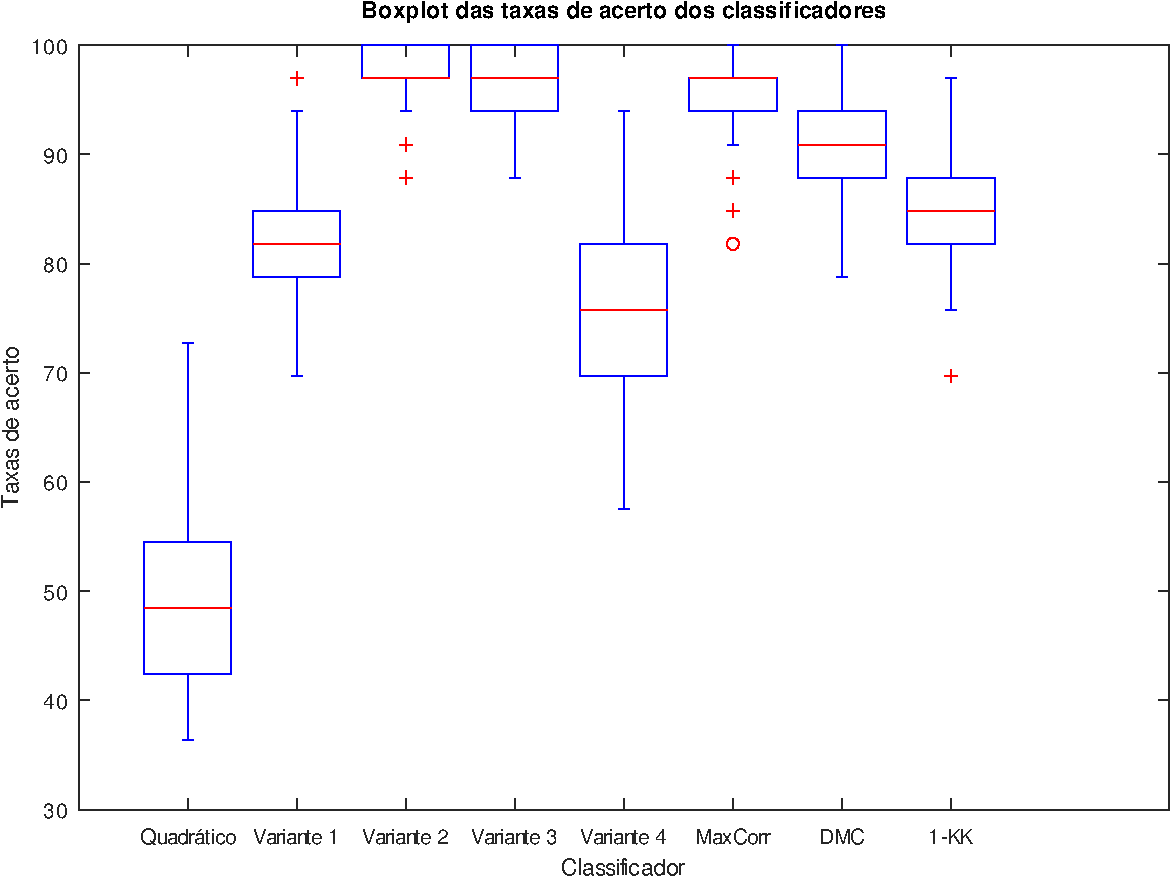
\includegraphics[width=0.7\textwidth]{figs/boxplot_pca_box.pdf}
    \caption{Boxplot dos resultados com PCA (com Box-Cox)}
\end{figure}

\nonumsubsection{Questão 7}
\begin{tcolorbox}[colback=blue!5!white, colframe=blue!75!black]
    Houve alguma mudança (melhora ou piora) nos desempenhos dos classifi-
cadores avaliados em relação aos resultados da Atividade 6? Quais classificadores
pioraram/melhoraram de desempenho com a aplicação da transformação BOX-COX
juntamente com PCA?
\end{tcolorbox}
A maioria dos classificadores tiveram uma leve piora nos resultados, mas nada muito significativo.
Os classificadores MaxCorr e DMC caíram 1 ponto percentual, e o 1-KK caiu 3 pontos percentuais.
O quadrático ainda teve dificuldade de condicionamento.

A variante 1 melhorou 3 pontos percentuais.
As variantes 2 e 3 melhoraram 2 pontos percentuais, Como essas duas variantes dependem da matriz de covariância
ponderada, o box-cox ajudou a melhorar o quão gaussiano são as classes. A variante 4 piorou 1 ponto percentual.

\nonumsection{Atividade 8}
\begin{tcolorbox}[colback=blue!5!white, colframe=blue!75!black]
    Projetar classificadores baseado em distância para aplicações de controle de
acesso. Modelo 1: Imagens vetorizadas + Classificador baseado em distância de Mahala-
nobis. Modelo 2: Imagens vetorizadas + PCA + normalização z-escore + Classificador
baseado em distância euclidiana. OBS: Adicione 11 imagens próprias ao conjunto de dados
para atuar como “intruso”; ou seja, indivíduo ao qual não deve ser dado acesso.
\end{tcolorbox}
Foram adicionadas 11 imagens de rostos da mesma pessoa, as imagens tiveram um preprocessamento para ficarem
em escala de cinza e em formato gif, além de terem sido redimensionadas para 20x20 pixels.

\nonumsubsection{Questão 8}
\begin{tcolorbox}[colback=blue!5!white, colframe=blue!75!black]
    Calcule os seguintes índices de desempenho para os classificadores implementados:
     acurácia, taxa de falsos negativos (proporção de pessoas às quais acesso foi permitido incorretamente)
      e taxa de falsos positivos (pessoas às quais acesso não foi permitido incorretamente), sensibilidade e precisão. Os valores devem ser médios com inclusão de medida de dispersão (e.g., desvio padrão) para 50 rodadas.
\end{tcolorbox}
Para o modelo 1, foi escolhida a variante 1 do classificador Quadrático,
 pois foi a que teve o melhor resultado e não teria problema com o condicionamento das matrizes. Além disso foi retirado o termo do probabilidade a priori da função discriminante.
Para o modelo 2, foi escolhido o classificador DMC, pois foi o que teve o melhor tempo de execução e bons resultados.
\begin{table}[H]
\centering
\begin{tabular}{|c|c|c|}%
\hline%
\textbf{Métrica}&\textbf{Média}&\textbf{Desvio Padrão}\\%
\hline%
\textbf{Acurácia}&98.4&2.3\\%
\hline%
\textbf{Falso Positivo}&1.7&2.5\\%
\hline%
\textbf{Falso Negativo}&0.0&0.0\\%
\hline%
\textbf{Sensibilidade}&100.0&0.0\\%
\hline%
\textbf{Precisão}&84.3&20.4\\%
\hline%
\end{tabular}
\caption{Resultados do Modelo 1.}
\end{table}
Na definição do limiar de decisão, foi calculada a maior distância entre os indivíduos internos e a menor distância entre os indivíduos intrusos dos valores de treino,
então foi retirada a média dessas duas distâncias e considerado o limiar de decisão. Se a distância do Classificador for maior que o limiar, o indivíduo é considerado intruso.

\begin{table}[H]
\centering
\begin{tabular}{|c|c|c|}%
\hline%
\textbf{Métrica}&\textbf{Média}&\textbf{Desvio Padrão}\\%
\hline%
\textbf{Acurácia}&98.6&1.8\\%
\hline%
\textbf{Falso Positivo}&0.9&1.8\\%
\hline%
\textbf{Falso Negativo}&10.0&22.6\\%
\hline%
\textbf{Sensibilidade}&90.0&22.6\\%
\hline%
\textbf{Precisão}&88.8&20.5\\%
\hline%
\end{tabular}
\caption{Resultados do Modelo 2.}
\end{table}

\end{document}